%% Creator: Inkscape inkscape 0.91, www.inkscape.org
%% PDF/EPS/PS + LaTeX output extension by Johan Engelen, 2010
%% Accompanies image file 'Aamodel.eps' (pdf, eps, ps)
%%
%% To include the image in your LaTeX document, write
%%   \input{<filename>.pdf_tex}
%%  instead of
%%   \includegraphics{<filename>.pdf}
%% To scale the image, write
%%   \def\svgwidth{<desired width>}
%%   \input{<filename>.pdf_tex}
%%  instead of
%%   \includegraphics[width=<desired width>]{<filename>.pdf}
%%
%% Images with a different path to the parent latex file can
%% be accessed with the `import' package (which may need to be
%% installed) using
%%   \usepackage{import}
%% in the preamble, and then including the image with
%%   \import{<path to file>}{<filename>.pdf_tex}
%% Alternatively, one can specify
%%   \graphicspath{{<path to file>/}}
%% 
%% For more information, please see info/svg-inkscape on CTAN:
%%   http://tug.ctan.org/tex-archive/info/svg-inkscape
%%
\begingroup%
  \makeatletter%
  \providecommand\color[2][]{%
    \errmessage{(Inkscape) Color is used for the text in Inkscape, but the package 'color.sty' is not loaded}%
    \renewcommand\color[2][]{}%
  }%
  \providecommand\transparent[1]{%
    \errmessage{(Inkscape) Transparency is used (non-zero) for the text in Inkscape, but the package 'transparent.sty' is not loaded}%
    \renewcommand\transparent[1]{}%
  }%
  \providecommand\rotatebox[2]{#2}%
  \ifx\svgwidth\undefined%
    \setlength{\unitlength}{829.38146728bp}%
    \ifx\svgscale\undefined%
      \relax%
    \else%
      \setlength{\unitlength}{\unitlength * \real{\svgscale}}%
    \fi%
  \else%
    \setlength{\unitlength}{\svgwidth}%
  \fi%
  \global\let\svgwidth\undefined%
  \global\let\svgscale\undefined%
  \makeatother%
  \begin{picture}(1,0.53657886)%
    \put(0,0){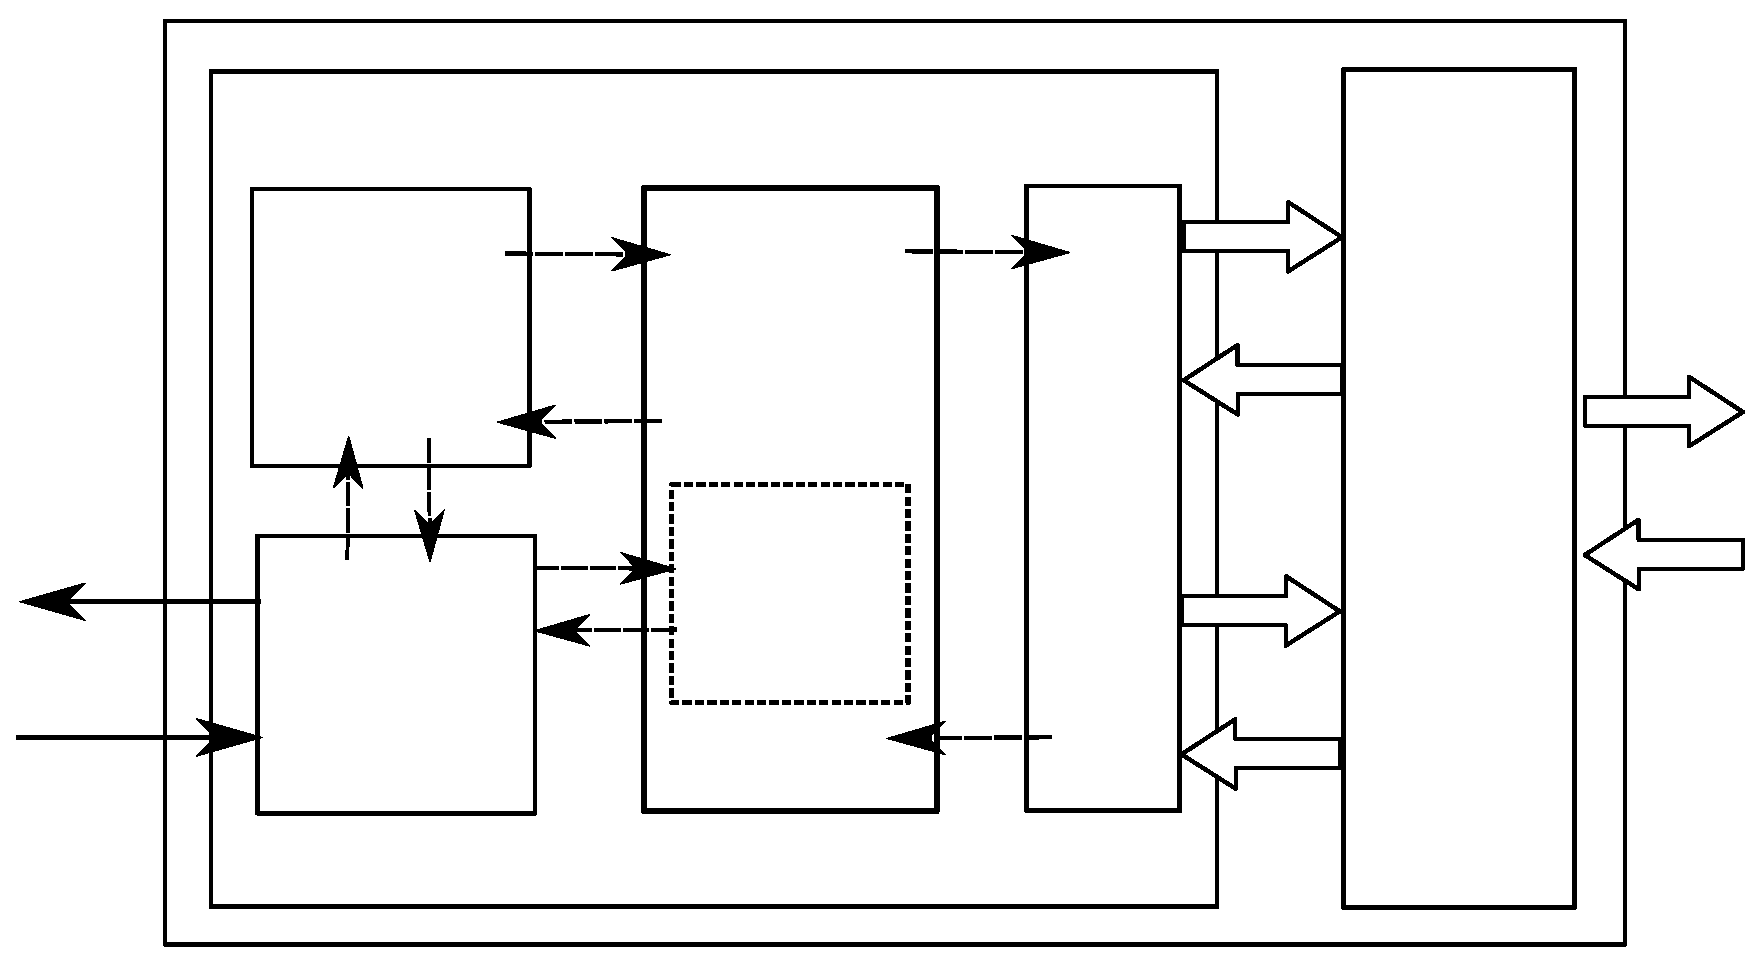
\includegraphics[width=\unitlength]{Aamodel.eps}}%
    \put(0.34212343,0.03143718){\makebox(0,0)[lb]{\smash{CPU core}}}%
    \put(0.17968158,0.34548351){\makebox(0,0)[lb]{\smash{CCU}}}%
    \put(0.41757325,0.34656825){\makebox(0,0)[lb]{\smash{TEU}}}%
    \put(0.599666914,0.25989433){\makebox(0,0)[lb]{\smash{MIU}}}%
    \put(0.7865488,0.22646533){\makebox(0,0)[lb]{\smash{\shortstack[lb]{Caches\\+\\MMU}}}}%
    \put(0.40472431,0.17360671){\makebox(0,0)[lb]{\smash{\shortstack[lb]{Debug\\ unit}}}}%
    \put(0.16260446,0.1291339){\makebox(0,0)[lb]{\smash{\shortstack[lb]{Debug\\ interface}}}}%
    \put(-0.0714272,0.13681176){\makebox(0,0)[lb]{\smash{\textit{\footnotesize\shortstack[lb]{Hardware\\debug link}}}}}%
  \end{picture}%
\endgroup%
